\documentclass[11pt,a4paper]{article}
\usepackage[T1]{fontenc}
\usepackage[utf8]{inputenc}
\usepackage{mathpazo}
\usepackage[margin=2.2cm]{geometry}
\usepackage{amsmath,amssymb}
\usepackage{enumitem}
\usepackage{xcolor}
\usepackage{titlesec}
\usepackage{booktabs,tabularx,longtable,array}
\usepackage[colorlinks=true,linkcolor=blue!50!black,urlcolor=blue!50!black]{hyperref}
\usepackage[capitalise,noabbrev]{cleveref}
\usepackage[most]{tcolorbox}
\usepackage{tikz}
\usetikzlibrary{arrows.meta,positioning,fit,calc,backgrounds,shapes.geometric}

\definecolor{navy}{HTML}{14213D}
\definecolor{blue}{HTML}{2E6F95}
\definecolor{orange}{HTML}{C96A1B}
\definecolor{okgreen}{HTML}{2E7D32}
\definecolor{skelamber}{HTML}{B7791F}
\definecolor{plangray}{HTML}{6B7280}
\titleformat{\section}{\Large\bfseries\color{navy}}{\thesection}{0.6em}{}
\titleformat{\subsection}{\large\bfseries\color{blue}}{\thesubsection}{0.5em}{}
\titleformat{\subsubsection}{\normalsize\bfseries\color{navy}}{\thesubsubsection}{0.5em}{}
\titlespacing*{\section}{0pt}{14pt}{6pt}
\titlespacing*{\subsection}{0pt}{10pt}{3pt}
\setlist{itemsep=2pt,topsep=3pt,leftmargin=1.4em}
\setlength{\parindent}{0pt}
\setlength{\parskip}{5pt}

\newtcolorbox{newc}[1]{colback=green!4,colframe=green!40!black,fonttitle=\bfseries\small,
  title={New concept: #1},boxrule=0.5pt,arc=2pt,left=5pt,right=5pt,top=3pt,bottom=3pt}
\newtcolorbox{incode}[1][]{colback=gray!5,colframe=gray!55,fonttitle=\bfseries\small,
  title={In the code#1},boxrule=0.5pt,arc=2pt,left=5pt,right=5pt,top=3pt,bottom=3pt,fontupper=\small}
\newtcolorbox{inprop}{colback=orange!5,colframe=orange!70!black,fonttitle=\bfseries\small,
  title={In the proposal},boxrule=0.5pt,arc=2pt,left=5pt,right=5pt,top=3pt,bottom=3pt,fontupper=\small}
\newtcolorbox{keybox}[1][]{colback=blue!5,colframe=blue!60!black,boxrule=0.6pt,arc=2pt,left=7pt,right=7pt,top=5pt,bottom=5pt,#1}

\newcommand{\done}{\textcolor{okgreen}{\textbf{[implemented]}}}
\newcommand{\skel}{\textcolor{skelamber}{\textbf{[skeleton]}}}
\newcommand{\planned}{\textcolor{plangray}{\textbf{[planned]}}}
\newcommand{\chk}{\textit{(check)}}
\newcommand{\code}[1]{{\small\ttfamily\begingroup\def\_{\textunderscore\allowbreak}\def\/{/\allowbreak}#1\endgroup}}
\emergencystretch=3em
\newcommand{\VC}{V^{C}}
\newcommand{\VW}{V^{W}}
\newcommand{\VS}{V^{S}}
\newcommand{\X}{\mathcal X}
\newcommand{\R}{\mathbb R}

\hypersetup{pdftitle={The scene digital twin: from data to referee}}

\begin{document}

\begin{center}
{\LARGE\bfseries\color{navy} The scene digital twin, from data to referee}\\[6pt]
{\large\color{navy} A step-by-step walkthrough of how the twin is built, stored and used, with the code}\\[8pt]
{\color{gray} Companion to the thesis proposal (27 Oct 2026), Steps 1--3 and their interfaces to Steps 4--9\\
Code: branch \code{twin}, commit \code{f4f669e} (17 Nov 2026) \quad·\quad written 25 Nov 2026}
\end{center}

\begin{keybox}[title={\textbf{How to read this document}},fonttitle=\color{white}\bfseries,colbacktitle=blue!60!black]
\begin{itemize}[leftmargin=1.2em]
\item \Cref{sec:what,sec:lifecycle} give the whole picture in two figures: what the twin is for, and the four moments at which it is built and used. Read these first.
\item \Cref{sec:data} lists every piece of data the twin needs and where it comes from. \Cref{sec:mujoco} explains the MuJoCo objects and answers ``how is the twin stored?''.
\item \Cref{sec:frames,sec:components} go through the components one by one, each with the proposal step it implements, the exact file and function, the data that goes in and out (with shapes), its status and its tests.
\item \Cref{sec:flow,sec:integration} follow one episode from the dataset to the trust weight, and show where the twin plugs into the training code.
\end{itemize}
Status tags: \done{} code exists and is tested; \skel{} interfaces exist, bodies raise \code{NotImplementedError}; \planned{} not in the repo yet (the roadmap work package is given). \chk{} marks statements I inferred but did not verify by running code. File paths are relative to the repo root; \code{RT/} abbreviates \code{third\_party\/rlinf\_runtime\/rlinf\/}. Green boxes introduce concepts that are new in these notes; orange boxes link to the proposal's symbols.
\end{keybox}

\tableofcontents
\newpage

%=====================================================================
\section{What the twin is, and what it is for}\label{sec:what}
%=====================================================================
The paper trains the policy (Cosmos) on rewards computed from Ctrl-World's \emph{imagined} video. The twin is a second, independent prediction of what the same actions do, produced by a completely different mechanism: rigid-body physics with contact in MuJoCo, instead of a learned video model. It is deliberately simple (a UR5 arm, a gripper, a laptop made of two boxes and a hinge, a table, three cameras). It is not meant to look real; it is meant to be \emph{physically consistent} and to \emph{know what it does not know}.

It is used as a referee. Wherever the twin is sure about what an action does and Ctrl-World disagrees, the reward computed from Ctrl-World's video is down-weighted. \Cref{fig:loop} shows where it sits.

\begin{figure}[h]
\centering
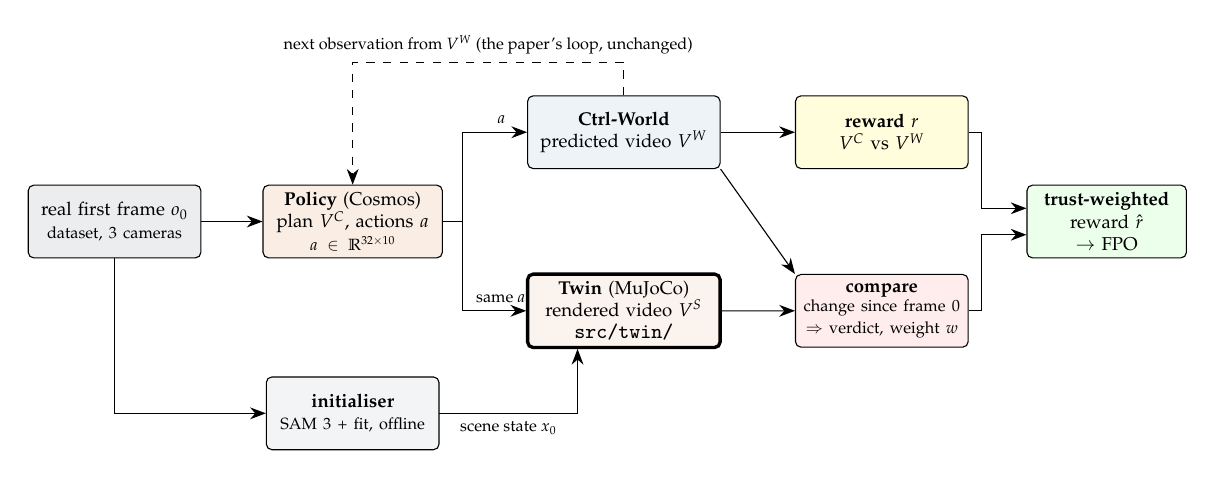
\begin{tikzpicture}[scale=0.84,transform shape,
  box/.style={draw,rounded corners=2pt,align=center,font=\footnotesize,minimum height=11mm,inner sep=3pt,text width=#1},
  box/.default=25mm, >={Stealth[length=2mm]}]
\node[box=24mm,fill=navy!8] (o0) at (0,0) {real first frame $o_0$\\ \scriptsize dataset, 3 cameras};
\node[box=25mm,fill=orange!12] (pol) at (3.6,0) {\textbf{Policy} (Cosmos)\\ plan $\VC$, actions $a$\\ \scriptsize $a\in\R^{32\times10}$};
\node[box=27mm,fill=blue!8] (wm) at (7.7,1.35) {\textbf{Ctrl-World}\\ predicted video $\VW$};
\node[box=27mm,fill=orange!8,very thick] (tw) at (7.7,-1.35) {\textbf{Twin} (MuJoCo)\\ rendered video $\VS$\\ \scriptsize \code{src/twin/}};
\node[box=24mm,fill=yellow!14] (rew) at (11.6,1.35) {\textbf{reward} $r$\\ $\VC$ vs $\VW$};
\node[box=24mm,fill=red!7] (cmp) at (11.6,-1.35) {\textbf{compare}\\ \scriptsize change since frame 0\\ $\Rightarrow$ verdict, weight $w$};
\node[box=22mm,fill=green!8] (tr) at (15.0,0) {\textbf{trust-weighted}\\ reward $\hat r$\\ $\to$ FPO};
\node[box=24mm,fill=navy!5] (ini) at (3.6,-2.9) {\textbf{initialiser}\\ \scriptsize SAM 3 + fit, offline};
\draw[->] (o0) -- (pol);
\draw[->] (pol.east) -- ++(3mm,0) |- (wm.west) node[pos=0.8,above,font=\scriptsize]{$a$};
\draw[->] (pol.east) -- ++(3mm,0) |- (tw.west) node[pos=0.8,above,font=\scriptsize]{same $a$};
\draw[->] (o0.south) |- (ini.west);
\draw[->] (ini.east) -| ([xshift=-7mm]tw.south) node[pos=0.25,below,font=\scriptsize]{scene state $x_0$};
\draw[->] (wm) -- (rew);
\draw[->] (wm.south east) -- (cmp.north west);
\draw[->] (tw) -- (cmp);
\draw[->] (rew.east) -- ++(2mm,0) |- ([yshift=2mm]tr.west);
\draw[->] (cmp.east) -- ++(2mm,0) |- ([yshift=-2mm]tr.west);
\draw[->,dashed] (wm.north) -- ++(0,5mm) -| node[pos=0.25,above,font=\scriptsize]{next observation from $\VW$ (the paper's loop, unchanged)} (pol.north);
\end{tikzpicture}
\caption{The paper's loop (top, unchanged) and the twin path (bottom, thick box). The twin starts once from the real first frame and from then on receives only the actions; it never sees generated frames.}
\label{fig:loop}
\end{figure}

\begin{inprop}
The twin is the object $\mathcal T$ of Step~1, eq.~(6); its initialisation is Step~2; running it is Step~3, eq.~(10), which produces $\VS_{i,k}(\vartheta)$. Everything downstream (Steps~4--8) only needs $\VS$ and a few twin states, so this document stops at the interface to Step~4 and shows how the pieces connect.
\end{inprop}

\textbf{What the twin can and cannot say.} It can say ``this imagined outcome is inconsistent with \emph{every} physical scene I consider plausible'' or ``it is consistent with \emph{some} plausible scene''. It cannot say ``this is what the real world does''; how close it is to reality is measured on real demonstrations (proposal Step~5.2, hypothesis H2).

%=====================================================================
\section{The life cycle: four moments}\label{sec:lifecycle}
%=====================================================================
The twin is not built in one go. Different parts are fixed at different moments, and each moment leaves a \emph{saved artefact} that the next one reads (\cref{fig:lifecycle}).

\begin{figure}[h]
\centering
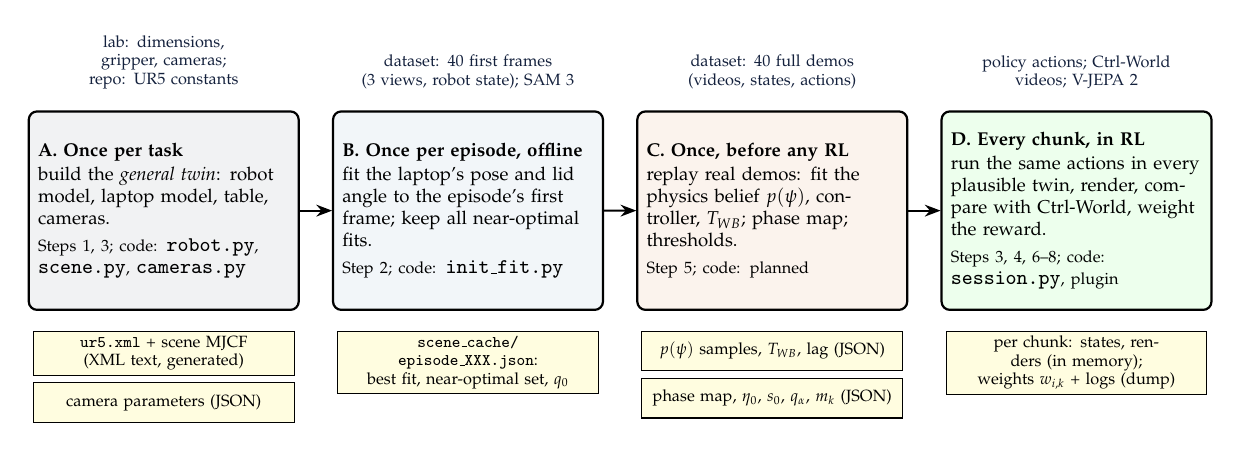
\begin{tikzpicture}[scale=0.84,transform shape,
  stage/.style={draw,rounded corners=3pt,thick,align=left,font=\footnotesize,text width=38mm,minimum height=30mm,anchor=north,inner sep=4pt},
  art/.style={draw,align=center,font=\scriptsize,fill=yellow!12,text width=38mm,inner sep=2pt,minimum height=6mm},
  inp/.style={align=center,font=\scriptsize,text width=38mm,text=navy},
  >={Stealth[length=2mm]}]
\node[stage,fill=navy!6] (A) at (0,0) {\textbf{A. Once per task}\\[1pt] build the \emph{general twin}: robot model, laptop model, table, cameras.\\[2pt] \scriptsize Steps 1, 3; code: \code{robot.py}, \code{scene.py}, \code{cameras.py}};
\node[stage,fill=blue!6] (B) at (4.6,0) {\textbf{B. Once per episode, offline}\\[1pt] fit the laptop's pose and lid angle to the episode's first frame; keep all near-optimal fits.\\[2pt] \scriptsize Step 2; code: \code{init\_fit.py}};
\node[stage,fill=orange!8] (C) at (9.2,0) {\textbf{C. Once, before any RL}\\[1pt] replay real demos: fit the physics belief $p(\psi)$, controller, $T_{WB}$; phase map; thresholds.\\[2pt] \scriptsize Step 5; code: planned};
\node[stage,fill=green!7] (D) at (13.8,0) {\textbf{D. Every chunk, in RL}\\[1pt] run the same actions in every plausible twin, render, compare with Ctrl-World, weight the reward.\\[2pt] \scriptsize Steps 3, 4, 6--8; code: \code{session.py}, plugin};
\node[inp,above=2mm of A] {lab: dimensions, gripper, cameras;\\ repo: UR5 constants};
\node[inp,above=2mm of B] {dataset: 40 first frames\\ (3 views, robot state); SAM 3};
\node[inp,above=2mm of C] {dataset: 40 full demos\\ (videos, states, actions)};
\node[inp,above=2mm of D] {policy actions; Ctrl-World\\ videos; V-JEPA 2};
\node[art,below=3mm of A] (a1) {\texttt{ur5.xml} + scene MJCF\\(XML text, generated)};
\node[art,below=1mm of a1] (a2) {camera parameters (JSON)};
\node[art,below=3mm of B] (b1) {\texttt{scene\_cache/}\\ \texttt{episode\_XXX.json}:\\ best fit, near-optimal set, $q_0$};
\node[art,below=3mm of C] (c1) {$p(\psi)$ samples, $T_{WB}$, lag (JSON)};
\node[art,below=1mm of c1] (c2) {phase map, $\eta_0$, $s_0$, $q_\alpha$, $m_k$ (JSON)};
\node[art,below=3mm of D] (d1) {per chunk: states, renders (in memory);\\ weights $w_{i,k}$ + logs (dump)};
\draw[->,thick] (A.east) -- (B.west);
\draw[->,thick] (B.east) -- (C.west);
\draw[->,thick] (C.east) -- (D.west);
\end{tikzpicture}
\caption{The four moments, what goes in (blue, above) and what is saved (yellow, below). A--C happen before training starts; only D runs inside the RL loop. Names of planned files are proposals.}
\label{fig:lifecycle}
\end{figure}

Two consequences worth keeping in mind:
\begin{itemize}
\item \textbf{Nothing expensive is decided inside the loop.} The scene fit (B) and the calibration (C) are done once and cached; the loop (D) only loads them. There are only 40 start scenes (32 training starts, 8 evaluation starts), so all 40 fits can be inspected by eye.
\item \textbf{The twin uses real data only.} B uses real first frames, C real demonstrations. Generated frames enter only at D, and only on the \emph{comparison} side, never to set the twin's state. That is what keeps the referee independent of the world model's mistakes (proposal \S5, ``No state is read from generated frames'').
\end{itemize}

%=====================================================================
\section{The data the twin needs}\label{sec:data}
%=====================================================================
\subsection{Inventory}
\begin{center}\small
\begin{tabularx}{\linewidth}{@{}>{\raggedright\arraybackslash}p{3.6cm}>{\raggedright\arraybackslash}X>{\raggedright\arraybackslash}p{2.4cm}>{\raggedright\arraybackslash}p{2.3cm}@{}}
\toprule
\textbf{Data} & \textbf{What it is, and what it is used for} & \textbf{Source} & \textbf{Status}\\
\midrule
UR5 kinematic constants, 0.18\,m TCP & DH table of the robot (\cref{sec:robot}); the twin must reproduce the function that produced Ctrl-World's conditioning states & repo, \code{eef\_pose\_adapter.py} & read, used (T1)\\
First frames of the 40 episodes & 3 images (\code{d405\_0\_rgb}, \code{d405\_1\_rgb}, \code{d435\_rgb}) and \code{observation.state}; input of the initialiser (B) and $q_0$ & LeRobot dataset \code{close\_desktop\_lerobot\_joint\_3cam} & \textbf{missing}\\
Full demonstrations (40) & videos, states, actions over time: calibration (C), demo replay check of T2, phase map & same dataset & \textbf{missing}\\
Action statistics (q01/q99) & gripper clip range used by production; probe range $\mathcal A_{\text{demo}}$ & file at \code{action\_stats\_path} & \textbf{missing}\\
Camera intrinsics & $K_v$ of the three RealSense cameras at the recorded resolution & lab (request 2) & \textbf{missing}\\
Camera extrinsics & $T_v$; or estimated from robot silhouettes in the demos (WP 3.3) & lab or estimated & \textbf{missing}\\
Laptop measurements & base and lid boxes, hinge position, maximum opening & lab (request 3) & placeholders\\
Gripper geometry & finger shape and opening; how the lid is pushed & lab (request 4) & placeholders\\
Robot confirmation & UR5 or UR5e, TCP offset, joint limits, controller & lab (request 5) & assumed UR5\\
Ctrl-World training episodes & which demos Ctrl-World was fine-tuned on (fair phase map) & lab / authors (request 6) & unknown\\
Model weights & SAM 3 (initialiser), V-JEPA 2 (comparison), Ctrl-World checkpoint (probes) & public / released & to install\\
\bottomrule
\end{tabularx}
\end{center}

\subsection{What is inside the dataset, and two open questions}
The env reads the dataset in \code{CtrlWorldEnv.reset} (\code{RT\/envs\/world\_model\/world\_model\_ctrl\_world\_env.py}, line~2050): for every reset episode it takes \code{episode\_data["start\_items"][0]}, the first frame, with its images and \code{observation.state}. The training and evaluation episodes are fixed in \code{src\/rlinf\_modified\/tasks.py}: 32 training ids and the 8 others ($\{6,7,14,20,26,31,32,37\}$) for evaluation. The dataset path in \code{configs/close.yaml} (line~179) is a placeholder, \code{\/path\/to\/shared\/datasets\/close\_desktop\_lerobot\_joint\_3cam}.

\begin{itemize}
\item \textbf{Joints or end-effector pose?} \code{observation.state} has 7 numbers, and two dataset formats in the code use the same layout: joints \code{[q0..q5, gripper]} or end-effector pose \code{[x, y, z, rx, ry, rz, gripper]}. Which one this dataset holds decides how the twin gets $q_0$ and the base transform $T_{WB}$ (\cref{sec:ik}). \code{progress.md} has a one-line check to run when the data arrives.
\item \textbf{Image size.} \code{cameras.py} records the dataset views as $480\times640$ and the loop views as $192\times320$ \chk. That resize is not aspect-preserving, so the intrinsics must be rescaled with the env's exact resize (or crop) rule.
\end{itemize}

\subsection{Which split is used for what}
\begin{center}\small
\begin{tabularx}{\linewidth}{@{}>{\raggedright\arraybackslash}p{2.8cm}>{\raggedright\arraybackslash}p{4.6cm}>{\raggedright\arraybackslash}X@{}}
\toprule
\textbf{Split} & \textbf{Episodes} & \textbf{Used for}\\
\midrule
RL starts & 32 training ids (\code{tasks.py}) & moment D: every group starts from one of these first frames\\
RL evaluation & 8 ids & evaluation rollouts of the policy\\
Initialiser (B) & all 40 first frames & one cached fit per episode\\
Calibration (C) & 40 demos, split 20 fit / 20 calibration & $p(\psi)$ and $m_k$ on the fit half; $q_\alpha$ on the calibration half\\
\bottomrule
\end{tabularx}
\end{center}

%=====================================================================
\section{MuJoCo in two pages, and how the twin is stored}\label{sec:mujoco}
%=====================================================================
\subsection{The three objects}
\begin{newc}{MJCF, \code{MjModel}, \code{MjData}}
MuJoCo separates what never changes during a simulation from what does.
\begin{itemize}[leftmargin=*]
\item \textbf{MJCF} is an XML text file describing the scene: bodies (rigid parts) nested in a tree, joints between them, geoms (shapes used for collision and drawing), sites (named points, e.g.\ the TCP), cameras, actuators (motors), and options such as the timestep.
\item \textbf{\code{mujoco.MjModel}} is the \emph{compiled} MJCF: flat numpy arrays of constants (masses, joint axes, friction, damping, camera poses, \ldots). It is built once with \code{mujoco.MjModel.from\_xml\_string(xml)}.
\item \textbf{\code{mujoco.MjData}} is the \emph{state} of one simulation of that model, plus everything computed from it: joint positions \code{qpos}, velocities \code{qvel}, actuator commands \code{ctrl}, time, body poses \code{xpos}/\code{xmat}, site poses, contacts. Created with \code{mujoco.MjData(model)}; many \code{MjData} can share one \code{MjModel}.
\item \textbf{\code{mujoco.mj\_step(model, data)}} advances \code{data} by one timestep; \code{mujoco.mj\_forward(model, data)} only recomputes derived quantities (poses, contacts) for the current \code{qpos} without moving time.
\end{itemize}
\end{newc}

\begin{figure}[h]
\centering
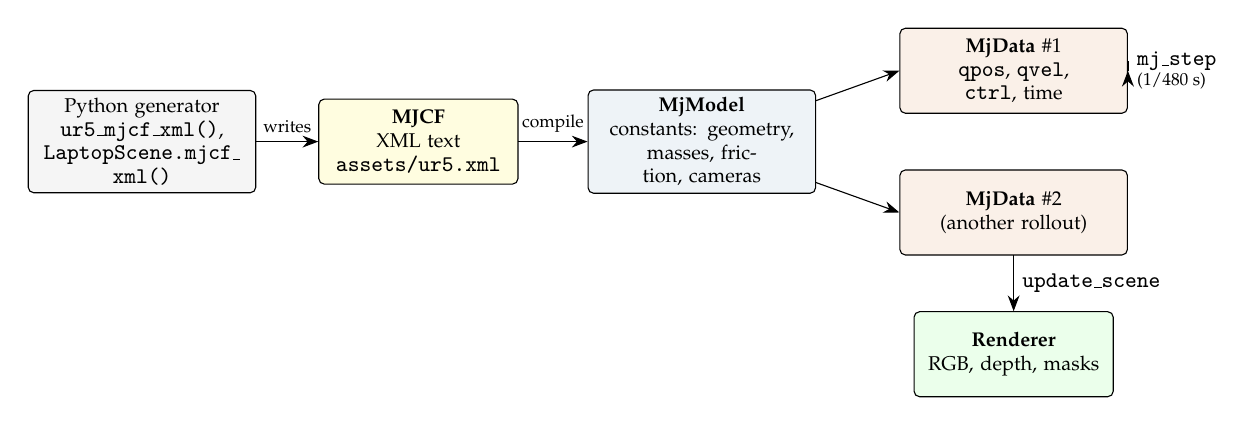
\begin{tikzpicture}[scale=0.9,transform shape,
  box/.style={draw,rounded corners=2pt,align=center,font=\footnotesize,minimum height=12mm,inner sep=3pt,text width=#1},
  box/.default=30mm, >={Stealth[length=2mm]}]
\node[box=30mm,fill=gray!8] (py) at (0,0) {Python generator\\ \code{ur5\_mjcf\_xml()},\\ \code{LaptopScene.mjcf\_xml()}};
\node[box=26mm,fill=yellow!12] (xml) at (3.9,0) {\textbf{MJCF}\\ XML text\\ \scriptsize\code{assets/ur5.xml}};
\node[box=30mm,fill=blue!8] (mod) at (7.9,0) {\textbf{MjModel}\\ constants: geometry,\\ masses, friction, cameras};
\node[box=30mm,fill=orange!10] (dat) at (12.3,1.0) {\textbf{MjData} \#1\\ \code{qpos}, \code{qvel}, \code{ctrl}, time};
\node[box=30mm,fill=orange!10] (dat2) at (12.3,-1.0) {\textbf{MjData} \#2\\ (another rollout)};
\node[box=26mm,fill=green!8] (ren) at (12.3,-3.0) {\textbf{Renderer}\\ RGB, depth, masks};
\draw[->] (py) -- node[above,font=\scriptsize]{writes} (xml);
\draw[->] (xml) -- node[above,font=\scriptsize]{compile} (mod);
\draw[->] (mod) -- (dat.west);
\draw[->] (mod) -- (dat2.west);
\draw[->,thick] (dat.east) to[out=20,in=-20,looseness=4] node[right,font=\scriptsize,align=left]{\code{mj\_step}\\ (1/480 s)} (dat.east);
\draw[->] (dat2.south) -- node[right,font=\scriptsize]{\code{update\_scene}} (ren.north);
\end{tikzpicture}
\caption{From generator code to images. The model is shared; each rollout has its own \code{MjData}.}
\label{fig:mujoco}
\end{figure}

\subsection{Where the twin's quantities live}
The proposal's uncertainty set $\Theta=\Psi_K\times\hat\X_\nu$ (eq.~9) maps onto these objects in a precise way, which decides how the code is organised:
\begin{itemize}
\item \textbf{Physics parameters $\psi$} (hinge friction and damping, friction coefficients, masses) are \emph{constants} of a simulation: they live in \code{MjModel} arrays (\code{dof\_frictionloss}, \code{dof\_damping}, \code{geom\_friction}, \code{body\_mass}). One $\psi$ $\Rightarrow$ one model, either a separate \code{MjModel} or the same one with these arrays overwritten before the rollout (for masses, derived constants may need recomputing with \code{mujoco.mj\_setConst} \chk).
\item \textbf{The start scene $x_0$} (laptop position, yaw, lid angle) and the robot joints $q_0$ are \emph{state}: they are entries of \code{MjData.qpos}.
\item \textbf{One element $\vartheta=(\psi,x_0)$} is therefore one (model, data) pair. With $K$ samples of $\psi$ and $M$ near-optimal fits, the twin runs $K\cdot M$ independent rollouts on the same actions (\cref{fig:theta}).
\end{itemize}

\begin{figure}[h]
\centering
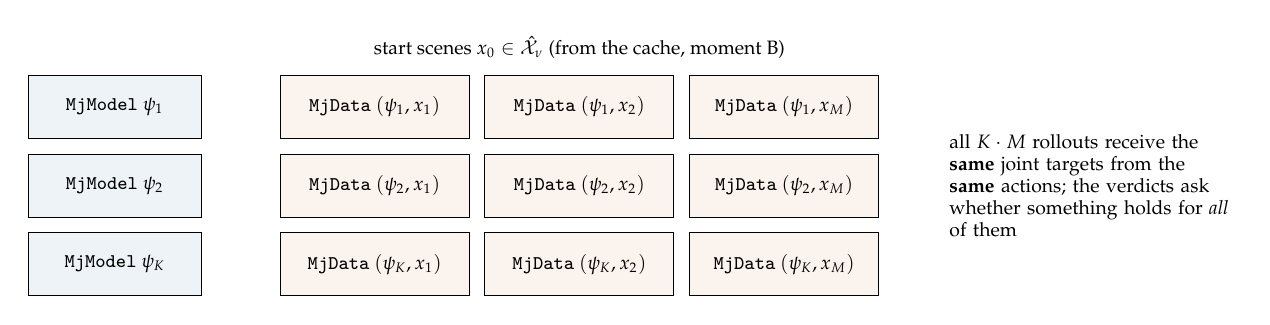
\begin{tikzpicture}[cell/.style={draw,minimum width=24mm,minimum height=8mm,font=\scriptsize,fill=orange!8},>={Stealth[length=2mm]}]
\foreach \r/\lab in {0/{\psi_1},1/{\psi_2},2/{\psi_K}}{
  \node[draw,fill=blue!8,font=\scriptsize,minimum width=22mm,minimum height=8mm,align=center] at (-1.4,-\r*1.0) {\texttt{MjModel} $\lab$};
  \foreach \c/\cl in {0/{x_1},1/{x_2},2/{x_M}}{
    \node[cell] at (1.9+\c*2.6,-\r*1.0) {\texttt{MjData} $(\lab,\cl)$};
  }
}
\node[font=\scriptsize,align=center] at (4.5,0.75) {start scenes $x_0\in\hat\X_\nu$ (from the cache, moment B)};
\node[font=\scriptsize,align=left,text width=36mm] at (11.0,-1.0) {all $K\cdot M$ rollouts receive the \textbf{same} joint targets from the \textbf{same} actions; the verdicts ask whether something holds for \emph{all} of them};
\end{tikzpicture}
\caption{The uncertainty set $\Theta$ as a grid of MuJoCo objects: rows share a model (one physics), columns share a start scene. The proposal subsamples $|\Theta|$ to about 16.}
\label{fig:theta}
\end{figure}

\subsection{So how is the twin saved?}
Not as one tensor. Each part is stored in the form that fits it:
{\small
\begin{longtable}{@{}>{\raggedright\arraybackslash}p{3.0cm}>{\raggedright\arraybackslash}p{3.3cm}>{\raggedright\arraybackslash}p{9.4cm}@{}}
\toprule
\textbf{Part} & \textbf{Form} & \textbf{Where, and why}\\
\midrule
\endhead
Robot model & MJCF text & \code{src\/twin\/assets\/ur5.xml}, committed, \emph{generated} by \code{scripts\/make\_twin\_ur5\_mjcf.py} from the DH table; a test checks the file equals the generator output, so it can never be hand-edited by mistake.\\
Scene model (robot + laptop + table + cameras) & MJCF string built in memory & \code{LaptopScene.mjcf\_xml()} \skel{} from \code{LaptopGeometry} and camera parameters; compiled at start-up. Can be dumped to a file for inspection (or saved as a binary \code{.mjb} with \code{mujoco.mj\_saveModel} \chk), but the source of truth is the generator plus its config.\\
Physics belief $p(\psi)$ & $K$ parameter dictionaries (JSON) & one file per task \planned{}; each sample is written into a model's arrays before a rollout.\\
Per-episode scene fit & JSON & \code{scene\_cache\/episode\_XXX.json} (\code{init\_fit.SCENE\_CACHE\_DIR}), not committed: best $x$, near-optimal set, IoU per view, $q_0$ (\code{EpisodeFit}).\\
Simulation state during a rollout & \code{MjData} in memory & never saved in normal use. A snapshot, e.g.\ for a probe that must restart from the same state, is a float64 vector: \code{mujoco.mj\_getState(model, data, buf, mujoco.mjtState.mjSTATE\_FULLPHYSICS)} and \code{mj\_setState} to restore \chk{} (names as in MuJoCo~3.x; confirm in 4.0.1). \code{copy.copy(data)} also duplicates an \code{MjData} \chk.\\
Per-chunk outputs & numpy arrays & joint path $(64,6)$, lid angle $(64,)$, contact flags $(64,)$ (\code{ChunkRollout}), renders as \code{uint8} arrays per camera. Streamed to the feature encoder, not stored (size: \cref{sec:size}).\\
Video features & torch tensors on GPU & V-JEPA 2 window features $\phi_t$, then the change features $c_t$ (Step~4).\\
Test fixtures & JSON & e.g.\ \code{tests\/fixtures\/twin\_fk\_reference\_ur5.json}; JSON because \code{.npz} is rejected by the repo's \code{scripts\/verify\_no\_weights.py}.\\
\bottomrule
\end{longtable}}

%=====================================================================
\section{Frames and conventions}\label{sec:frames}
%=====================================================================
Most twin bugs are convention bugs, so the conventions are fixed in \code{CLAUDE.md} and \code{src\/twin\/transforms.py}.

\begin{newc}{homogeneous transform $T_{AB}$}
A $4\times4$ matrix $\begin{bmatrix}R&p\\0&1\end{bmatrix}$ with $R$ a rotation matrix and $p$ a translation. $T_{AB}$ maps coordinates expressed in frame $B$ into frame $A$: a point $p_B$ becomes $p_A=Rp_B+p$. Transforms chain by matrix product, $T_{AC}=T_{AB}\,T_{BC}$, and $T_{BA}=T_{AB}^{-1}$ (\code{transforms.invert\_T}).
\end{newc}

\begin{figure}[h]
\centering
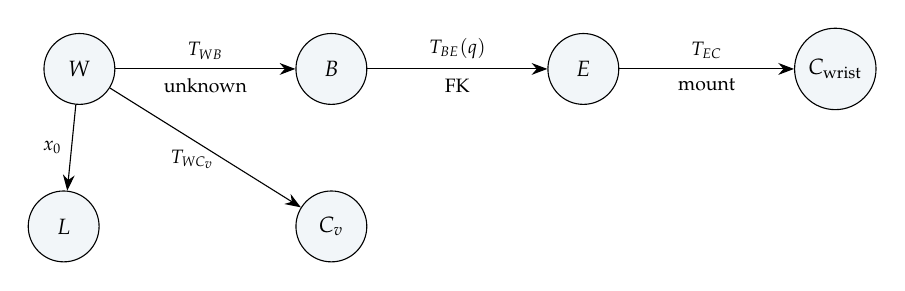
\begin{tikzpicture}[fr/.style={draw,circle,minimum size=9mm,font=\footnotesize,fill=blue!6},>={Stealth[length=2mm]}]
\node[fr] (W) at (0,0) {$W$};
\node[fr] (B) at (3.2,0) {$B$};
\node[fr] (E) at (6.4,0) {$E$};
\node[fr] (Cw) at (9.6,0) {$C_{\text{wrist}}$};
\node[fr] (Cf) at (3.2,-2.0) {$C_{v}$};
\node[fr] (L) at (-0.2,-2.0) {$L$};
\draw[->] (W) -- node[above,font=\scriptsize]{$T_{WB}$} node[below,font=\scriptsize]{unknown} (B);
\draw[->] (B) -- node[above,font=\scriptsize]{$T_{BE}(q)$} node[below,font=\scriptsize]{FK} (E);
\draw[->] (E) -- node[above,font=\scriptsize]{$T_{EC}$} node[below,font=\scriptsize]{mount} (Cw);
\draw[->] (W) -- node[left,font=\scriptsize,pos=0.6]{$T_{WC_v}$} (Cf);
\draw[->] (W) -- node[left,font=\scriptsize]{$x_0$} (L);
\end{tikzpicture}
\caption{The frames. $W$: frame of the recorded end-effector poses (and of Ctrl-World's state); $B$: robot base; $E$: TCP; $C_v$: fixed cameras; $C_{\text{wrist}}$: wrist camera, rigid on $E$; $L$: laptop base, posed by the scene state $x_0$; the lid is $L$ rotated about the hinge by $\vartheta$.}
\label{fig:frames}
\end{figure}

\begin{center}\small
\begin{tabularx}{\linewidth}{@{}>{\raggedright\arraybackslash}p{3.8cm}>{\raggedright\arraybackslash}X@{}}
\toprule
\textbf{Quantity} & \textbf{Convention (verified by reading the repo)}\\
\midrule
EEF state (repo, Ctrl-World) & $[x,y,z,r_x,r_y,r_z,\text{gripper}]$ in $W$, rotation as an \emph{axis-angle vector} (direction = axis, length = angle)\\
Action (policy) & 10 numbers per step: position delta (3), rotation delta as rot6d (6: the first two columns of a rotation matrix), absolute gripper (1); chained in the \emph{body frame}: $T_{i+1}=T_i\,\Delta T$, gains 1.0\\
Inside the twin & rotations as $3\times3$ matrices; axis-angle only at the boundary (\code{rotvec\_to\_matrix}, \code{so3\_log}); rotations compared by geodesic angle (\code{geodesic\_angle}, via \code{atan2} for accuracy near 0 and $\pi$)\\
rot6d & never converted by twin code: the repo function is imported by file path (\code{repo\_import.load\_eef\_pose\_adapter})\\
Camera names & by physical camera: main = \code{d405\_0\_rgb}, wrist = \code{d435\_rgb}, side = \code{d405\_1\_rgb} (\code{cameras.PHYSICAL\_CAMERAS})\\
\bottomrule
\end{tabularx}
\end{center}

%=====================================================================
\section{The components, one by one}\label{sec:components}
%=====================================================================
Each subsection follows the same order: what it does, the proposal step, the code, inputs and outputs, tests.

%---------------------------------------------------------------------
\subsection{Robot model (milestone T1) \done}\label{sec:robot}
\textbf{What it does.} Gives the pose of the TCP for any joint angles, $T_{BE}(q)$, exactly as the repo function that produced Ctrl-World's conditioning states, and a MuJoCo model of the same arm.

\begin{newc}{Denavit--Hartenberg (DH) parameters}
A compact way to describe a serial arm: each joint $i$ contributes a fixed transform built from 4 numbers, $T_{i-1,i}=R_z(q_i)\,T_z(d_i)\,T_x(a_i)\,R_x(\alpha_i)$, where $q_i$ is the joint angle and $(a_i,d_i,\alpha_i)$ are constants of the robot. The TCP pose is the product of the six link transforms and a fixed tool offset.
\end{newc}

\begin{incode}[: \code{src/twin/robot.py}]
\begin{itemize}[leftmargin=*]
\item \code{UR5\_DH}: the six $(a,d,\alpha)$ rows read from the repo FK (\code{RT\/envs\/world\_model\/eef\_pose\_adapter.py}): $d_1=0.089159$, $a_2=-0.425$, $a_3=-0.39225$, $d_4=0.10915$, $d_5=0.09465$, $d_6=0.0823$\,m, twists $(\pi/2,0,0,\pi/2,-\pi/2,0)$. \code{TCP\_OFFSET} $=(0,0,0.18)$\,m. These are the original UR5, not the UR5e.
\item \code{fk(q)}: batched numpy FK, $(\ldots,6)\to(\ldots,4,4)$.
\item \code{ur5\_mjcf\_xml()}: writes the MJCF. Each body frame is placed \emph{on its own joint axis} (hinge about $+z$, \code{qpos} $=q$, no offsets), which avoids the usual DH-versus-MuJoCo axis mistake. Sites \code{flange} and \code{tcp}. \code{compiler angle="radian"} is explicit (MJCF defaults to degrees).
\item \code{load\_ur5\_model()}: \code{mujoco.MjModel.from\_xml\_string(ur5\_mjcf\_xml())}.
\item Link geoms are visual-only capsules with nominal masses (no collision yet; contact comes with T3).
\end{itemize}
\end{incode}

\textbf{Tests.} \code{tests/test\_twin\_fk.py} and \code{test\_twin\_mujoco\_fk.py}: over 1000 random joint vectors, numpy FK and MuJoCo's \code{tcp} site equal the repo FK to $7\times10^{-16}$\,m and $8\times10^{-14}$\,rad (acceptance $10^{-5}$). The reference table is generated once from the repo function in float64 by \code{scripts/make\_twin\_fk\_reference.py}; a staleness test regenerates it when torch is present.

%---------------------------------------------------------------------
\subsection{From actions to end-effector targets (milestone T2) \done}\label{sec:actions}
\textbf{What it does.} Converts one policy chunk into the 64 end-effector targets that Ctrl-World is conditioned on, \emph{bit for bit}. Both models must follow the same commanded path, otherwise a disagreement could be a conversion artefact.

\begin{figure}[h]
\centering
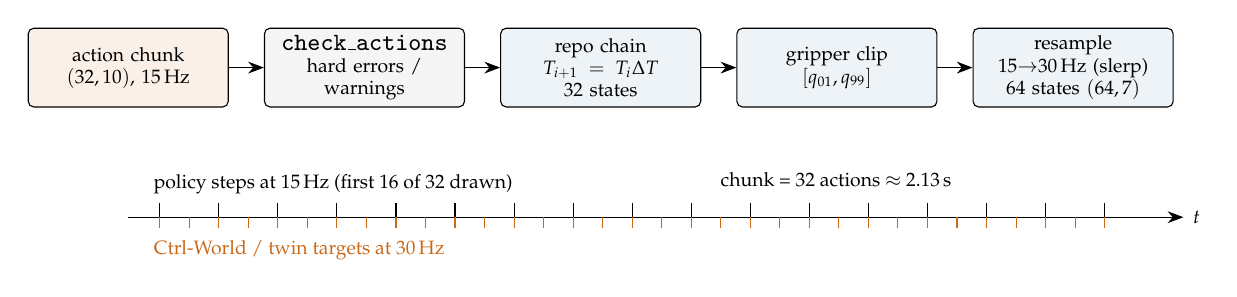
\begin{tikzpicture}[>={Stealth[length=2mm]},
  st/.style={draw,rounded corners=2pt,align=center,font=\scriptsize,minimum height=10mm,text width=24mm,inner sep=2pt}]
\node[st,fill=orange!10] (a) at (0,0) {action chunk\\ $(32,10)$, 15\,Hz};
\node[st,fill=gray!8] (c) at (3.0,0) {\code{check\_actions}\\ hard errors /\\ warnings};
\node[st,fill=blue!8] (r) at (6.0,0) {repo chain\\ $T_{i+1}=T_i\Delta T$\\ 32 states};
\node[st,fill=blue!8] (g) at (9.0,0) {gripper clip\\ $[q_{01},q_{99}]$};
\node[st,fill=blue!8] (s) at (12.0,0) {resample\\ 15$\to$30\,Hz (slerp)\\ 64 states $(64,7)$};
\draw[->] (a)--(c); \draw[->] (c)--(r); \draw[->] (r)--(g); \draw[->] (g)--(s);
% time grid
\begin{scope}[yshift=-1.9cm]
\draw[->] (0,0) -- (13.4,0) node[right,font=\scriptsize]{$t$};
\foreach \i in {0,...,16}{ \draw (0.4+\i*0.75,0) -- ++(0,0.18); }
\foreach \i in {0,...,32}{ \draw[orange] (0.4+\i*0.375,0) -- ++(0,-0.14); }
\node[font=\scriptsize,anchor=west] at (0.2,0.42) {policy steps at 15\,Hz (first 16 of 32 drawn)};
\node[font=\scriptsize,anchor=west,text=orange] at (0.2,-0.42) {Ctrl-World / twin targets at 30\,Hz};
\node[font=\scriptsize,align=left,anchor=west] at (7.4,0.48) {chunk = 32 actions $\approx$ 2.13\,s};
\end{scope}
\end{tikzpicture}
\caption{The T2 pipeline for one chunk, and the two time grids. Everything in blue is the repo's own code, imported by file path and run in float32 exactly as in production.}
\label{fig:actions}
\end{figure}

\begin{incode}[: \code{src/twin/actions.py}]
\begin{itemize}[leftmargin=*]
\item \code{check\_actions(actions)}: shape, non-finite values and degenerate rot6d are hard errors; large steps, rot6d far from orthonormal, gripper out of range are warnings (\code{ActionReport}).
\item \code{actions\_to\_eef\_targets(current\_state, actions)} returns \code{EEFTargets}: \code{policy\_states} $(B,32,7)$, \code{ctrl\_states} $(B,64,7)$, \code{ctrl\_condition} $(B,64,7)$ (what Ctrl-World is conditioned on: the current state plus the first 63) and \code{next\_state} $(B,7)$ (where the next chunk starts). It calls \code{analytic\_ur5\_rot6d\_delta\_actions\_to\_eef\_states}, \code{state\_to\_ctrl\_world\_eef\_state} and \code{resample\_eef\_state\_sequence\_by\_fps} from the repo.
\item \code{AdapterConfig}: the resolved production settings (gains 1.0, body frame, 15/30\,Hz, internal rollout). \code{gripper\_clip} is \code{None} until the action statistics are available.
\item Production counterpart: \code{CtrlWorldEnv.\_convert\_via\_analytic\_ur5\_rot6d} (\code{world\_model\_ctrl\_world\_env.py}, line~1599). \code{tests/test\_twin\_actions.py} calls that production method on a stand-in object and checks bit-equality.
\end{itemize}
\end{incode}

\textbf{One design choice to remember.} The twin carries the end-effector state \emph{open loop}, exactly like Ctrl-World (\code{next\_state}), not by forward kinematics of its own joints. Both models then follow the same commanded path; if the arm cannot follow it, that shows up as IK flags, not as a slow drift between the two.

%---------------------------------------------------------------------
\subsection{From end-effector targets to joint targets (milestone T2) \done}\label{sec:ik}
\textbf{What it does.} Maps the 64 targets from frame $W$ to the robot base ($T_{BE}=T_{WB}^{-1}T_{WE}$) and solves inverse kinematics (IK) for each, giving 64 joint vectors the simulated arm will track.

\begin{newc}{inverse kinematics by damped least squares}
IK finds joint angles $q$ whose FK equals a target pose. The \emph{Jacobian} $J(q)$ ($6\times6$) linearises FK: a small joint change $\Delta q$ moves the TCP by $J\Delta q$ (3 linear + 3 angular components). Newton-style IK repeats $\Delta q=J^{-1}e$ with $e$ the pose error. Near a \emph{singularity} (arm stretched, wrist aligned) $J$ is almost not invertible and $J^{-1}e$ explodes; \emph{damped} least squares uses $\Delta q=V\,\mathrm{diag}\!\big(\tfrac{s}{s^2+\lambda^2}\big)U^\top e$ (from the SVD $J=U\,\mathrm{diag}(s)V^\top$), which limits the step where a singular value $s$ is small.
\end{newc}

\begin{incode}[: \code{src/twin/ik.py} and \code{actions.ActionsToJoints}]
\begin{itemize}[leftmargin=*]
\item \code{jacobian(q)}: geometric Jacobian at the TCP; equals finite differences and MuJoCo's \code{mj\_jacSite} to $10^{-12}$.
\item \code{ik\_analytic(T\_BE)}: the closed-form UR5 solutions (up to 8 branches: shoulder $\times$ elbow $\times$ wrist). Used to choose the \emph{initial} configuration when only an EEF pose is known (\code{initial\_configuration}).
\item \code{ik\_dls(T, q\_seed)}: damped least squares from a warm start, with damping that switches on only near a singularity and fades as the error goes to zero.
\item \code{track\_path(T\_targets, q\_start, dt)}: seeds each frame with the previous solution, so the path stays on one branch, and returns \code{PathIKResult} with per-frame flags: \code{converged}, \code{at\_limit}, \code{speed\_violation} (180\,deg/s, \chk), \code{branch\_switch}, \code{min\_singular\_value}. \code{feasible} is all of them clean.
\item \code{ActionsToJoints(T\_WB).step\_chunk(state, actions, q)} chains everything and returns a \code{JointChunk}: \code{q} $(64,6)$, \code{gripper} $(64,)$, the \code{EEFTargets}, the action report, the IK result and \code{next\_state}. $T_{WB}$ is the identity placeholder until it is estimated (moment C) or given by the lab.
\end{itemize}
\end{incode}

\textbf{Tests.} \code{test\_twin\_ik.py}, \code{test\_twin\_action\_to\_joints.py}: FK(IK) within $10^{-6}$\,m/rad over five chained chunks, also with an offset $T_{WB}$. The \emph{real} check (recorded actions converted and compared with recorded states of the following frames) needs the dataset: it is the first thing to run when the data arrives, because it is the only guard against an error in the shared conversion, which by construction the twin cannot detect.

\begin{inprop}
Together, \cref{sec:actions,sec:ik} are the action conversion $T_S$ of Step~3 (``inverse kinematics of the relative end-effector motion''). The IK feasibility flags are also the robot-twin part of the probe admissibility set $\mathcal A_{\text{feas}}$ of Step~6.2 (reachable, within limits).
\end{inprop}

%---------------------------------------------------------------------
\subsection{The physical scene (milestone T3) \skel}\label{sec:scene}
\textbf{What it does.} Adds the laptop, the table and the gripper fingers to the arm, and simulates contact: the 64 joint targets of a chunk drive the arm, the fingers push the lid, physics decides what the lid does.

\begin{incode}[: \code{src/twin/scene.py} (interfaces exist; bodies raise \code{NotImplementedError})]
\begin{itemize}[leftmargin=*]
\item \code{LaptopGeometry}: base and lid box sizes, hinge offset, maximum opening (placeholders for a 13--15 inch laptop until lab request 3).
\item \code{PhysicsParams}: one $\psi$: hinge \code{frictionloss}, \code{damping}, \code{armature}, lid mass and centre of mass, base mass, finger--lid and base--table friction, contact softness (\code{solref}, \code{solimp}), controller lag.
\item \code{GripperModel}: map from the absolute gripper value (dataset units, clip range $[q_{01},q_{99}]$) to finger opening in metres.
\item \code{SceneState}: $x=(p_x,p_y,\text{yaw},\vartheta)$ plus arm joints and gripper; \code{ChunkRollout}: per-frame states, lid angle $(64,)$, finger--lid contact flags $(64,)$, maximum penetration $(64,)$.
\item \code{LaptopScene}: \code{mjcf\_xml()}, \code{reset(state)}, \code{step\_chunk(q\_targets, gripper)}, \code{get\_state()}. Constants: \code{PHYSICS\_TIMESTEP} $=1/480$\,s, \code{SUBSTEPS\_PER\_FRAME} $=16$ (16 physics steps per 30\,Hz frame).
\end{itemize}
\end{incode}

\textbf{How \code{step\_chunk} will work} \planned{} (WP 2.3):
\begin{enumerate}
\item The arm gets \emph{position actuators} on its six joints: \code{data.ctrl} is set to the joint target of the current 30\,Hz frame, and a spring--damper inside MuJoCo pulls the joint towards it. This gives finite contact forces, like a real controller (setting \code{qpos} directly would make the arm infinitely stiff and contacts violent).
\item For each of the 64 frames: set \code{ctrl} (arm) and the finger opening, call \code{mj\_step} 16 times, record the lid hinge angle from \code{qpos}, the finger--lid contacts from \code{data.contact}, and the deepest penetration.
\item \code{reset(state)}: write $q_0$ and $x_0$ into \code{qpos}, zero velocities, hold the arm and let contacts settle briefly; reject the state if anything keeps moving (Step 2.3, ``physical check'').
\end{enumerate}

\begin{newc}{why the hinge friction has a lower bound}
A real lid stays where you leave it because dry friction in the hinge holds it against gravity. In the twin this is \code{frictionloss}; it must exceed the gravity torque of the lid over the working range, or the lid falls shut with no robot contact. A twin with too little friction would ``agree'' with an imagined video in which the lid closes by itself, exactly the failure the referee must catch. So parameter samples under which the observed start would move are discarded for that scene (proposal Step 3), and the null-action test (P8) checks it: zero commanded motion must leave every body still.
\end{newc}

\textbf{Planned MuJoCo layout.} \code{qpos} would contain: 6 arm hinges, the laptop base's free joint (7 numbers: position and a unit quaternion), the lid hinge (1), and the finger joints (0 or 2, depending on the gripper mode) \planned. Acceptance tests are written in the \code{scene.py} docstring: scripted close shuts the lid; null action $<10^{-6}$\,m drift after 5\,s; deterministic; stable for 200 parameter draws; halving the timestep changes the final lid angle by $<0.5^\circ$.

%---------------------------------------------------------------------
\subsection{Cameras and rendering (milestones T0, T4) \skel}\label{sec:render}
\textbf{What it does.} Renders what the three real cameras would see of the twin: colour images to compare with Ctrl-World's video, and segmentation masks for the initialiser.

\begin{incode}[: \code{src/twin/cameras.py}, \code{src/twin/render.py}]
\begin{itemize}[leftmargin=*]
\item \code{CameraIntrinsics} ($f_x,f_y,c_x,c_y$, size) with \code{resized(h, w)}; its docstring warns that $480\times640\to192\times320$ is not aspect-preserving.
\item \code{Camera}: name, intrinsics, \code{T\_WC} (or $T_{EC}$ for the wrist camera, \code{attached\_to\_eef}).
\item \code{project(K, T\_WC, p\_W)}: pinhole projection of 3D points to pixels (OpenCV axes: $x$ right, $y$ down, $z$ forward).
\item \code{TwinRenderer.render(data, camera)} (T0) and \code{render\_masks(data, camera)} (T4) are stubs. A one-off EGL render at $192\times320$ worked on the lab workstation.
\end{itemize}
\end{incode}

\textbf{How it will work} \planned{} (WP 1.1, 3.1). The cameras become MJCF \code{<camera>} elements built from $(K_v,T_v)$. MuJoCo cameras look along their $-z$ axis with $y$ up, so the OpenCV pose is converted with $\mathrm{diag}(1,-1,-1)$ \chk. The wrist camera is a child of the end-effector body, so it moves with the arm. A \code{mujoco.Renderer(model, 192, 320)} then gives RGB with \code{update\_scene(data, camera=name)} and \code{render()}; with segmentation rendering enabled it returns, per pixel, the id of the geom it shows, from which masks of robot, base and lid follow.

\textbf{Texture.} To reduce the visual gap, the real first frame is projected onto the twin's objects as texture (proposal Step 3, ``Rendering''): at $t=0$ the render nearly reproduces the real image, later frames show those surfaces moving. This only matters for the V-JEPA comparison; the masks do not depend on it.

%---------------------------------------------------------------------
\subsection{The initialiser (milestone T5) \skel}\label{sec:init}
\textbf{What it does.} Finds, for each episode, the laptop state $x_0$ that explains its first frame, and keeps every fit that is nearly as good as the best one.

\begin{figure}[h]
\centering
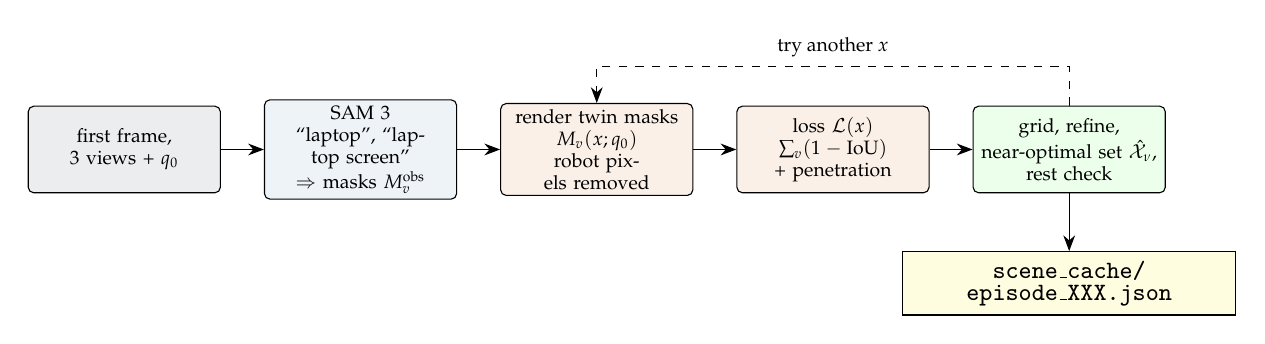
\begin{tikzpicture}[>={Stealth[length=2mm]},
  st/.style={draw,rounded corners=2pt,align=center,font=\scriptsize,minimum height=11mm,text width=23mm,inner sep=2pt}]
\node[st,fill=navy!8] (f) at (0,0) {first frame,\\ 3 views + $q_0$};
\node[st,fill=blue!8] (m) at (3.0,0) {SAM 3\\ ``laptop'', ``laptop screen''\\ $\Rightarrow$ masks $M^{\text{obs}}_v$};
\node[st,fill=orange!10] (r) at (6.0,0) {render twin masks\\ $M_v(x;q_0)$\\ robot pixels removed};
\node[st,fill=orange!10] (l) at (9.0,0) {loss $\mathcal L(x)$\\ $\sum_v(1-\mathrm{IoU})$\\ + penetration};
\node[st,fill=green!8] (s) at (12.0,0) {grid, refine,\\ near-optimal set $\hat\X_\nu$,\\ rest check};
\node[draw,fill=yellow!12,font=\scriptsize,align=center,text width=40mm] (j) at (12.0,-1.7) {\code{scene\_cache\/episode\_XXX.json}};
\draw[->] (f)--(m); \draw[->] (m)--(r); \draw[->] (r)--(l); \draw[->] (l)--(s); \draw[->] (s)--(j);
\draw[->,dashed] (s.north) -- ++(0,0.5) -| node[pos=0.25,above,font=\scriptsize]{try another $x$} (r.north);
\end{tikzpicture}
\caption{Render-and-compare fit of Step 2. It runs offline, once per episode; the loop only reads the cached JSON.}
\label{fig:init}
\end{figure}

\begin{newc}{render-and-compare, near-optimal set}
Instead of reading the laptop's pose from the image with a learned detector, the fitter \emph{guesses} a pose, renders the twin's laptop from each calibrated camera, and measures how well the rendered silhouettes overlap the SAM 3 masks (IoU, intersection over union, in $[0,1]$). It searches for the pose with the best overlap. Because a few silhouettes can be ambiguous (a lid seen edge-on, a nearly symmetric base), it keeps \emph{all} poses whose loss is within a tolerance $\nu$ of the best: the near-optimal set $\hat\X_\nu$ (proposal eq.~8). Later verdicts must hold for all of them.
\end{newc}

\begin{incode}[: \code{src/twin/init\_fit.py}]
\code{EpisodeFit} holds \code{episode\_id}, \code{best} and \code{near\_optimal} (\code{SceneState}s), \code{iou\_per\_view} and \code{q0}. \code{fit\_episode(episode\_id)} and \code{load\_cached\_fit(episode\_id)} are stubs; the cache folder is \code{SCENE\_CACHE\_DIR = scene\_cache/}. The roadmap (WP 3.2) adds a \code{TaskConfig} (prompts, object model, unknowns and ranges) so the same code serves the four tasks of G1, and tests the fit on synthetic renders with known answers before real frames exist.
\end{incode}

%---------------------------------------------------------------------
\subsection{The physics belief and calibration (proposal Step 5) \planned}\label{sec:calib}
\textbf{What it does.} Fixes everything the twin does not know from first principles, using real demonstrations only, before any RL run:
\begin{itemize}
\item \textbf{$p(\psi)$}: replay each fit-half demonstration in the twin (first frame from the initialiser, recorded actions through T2), and keep the parameter values whose rendered change matches the real video's change. The result is a set of $K$ samples (about 16 used per rollout).
\item \textbf{$T_{WB}$, controller lag and gains}: from commanded versus recorded robot states.
\item \textbf{Phase map}: in which phases (free motion, contact, after contact) the twin is closer to the real video than Ctrl-World. The twin is consulted only there.
\item \textbf{Thresholds}: appearance floor $\eta_0$ and $\eta=2\eta_0$, Ctrl-World significance $s_0$, divergence scale $m_k$ and conformal threshold $q_\alpha$ (computed on the calibration half).
\end{itemize}
All of these are small and are saved as JSON next to the scene cache (file names to be fixed; roadmap WP 1.5, 3.4).

%---------------------------------------------------------------------
\subsection{The per-environment session (milestone T7) \skel}\label{sec:session}
\textbf{What it does.} Holds the twin of one environment of the RL loop through an episode: reset at the episode's start, one step per chunk with that environment's actions.

\begin{incode}[: \code{src/twin/session.py}]
\code{TwinSession(actions\_to\_joints, scene=None)} works today in \emph{kinematics-only} mode: \code{reset(eef\_state, q0)} and \code{step\_chunk(actions)} run checks, EEF targets and IK, and keep the open-loop EEF state and the last joint vector; \code{reachability\_summary()} reports the share of chunks with IK failure, limit hits, speed violations, branch switches and action warnings. With a \code{scene}, \code{step\_chunk} also calls \code{scene.step\_chunk} and stores the \code{ChunkRollout} in a \code{ChunkResult} (which also has a \code{renders} dict per camera).
\end{incode}

\textbf{What it must become} \planned: one session holds the $K\cdot M$ (model, data) pairs of \cref{fig:theta}. The joint targets are computed \emph{once} per chunk (they do not depend on $\psi$ or $x_0$, only on the actions and the start joints) and fed to every pair; each pair returns its \code{ChunkRollout} and renders. That is eq.~(10) of the proposal for all $\vartheta\in\Theta$.

%=====================================================================
\section{End to end: one episode, from the dataset to the weight}\label{sec:flow}
%=====================================================================
\Cref{fig:flow} puts the components together. The left half runs before training, the right half in every chunk.

\begin{figure}[h]
\centering
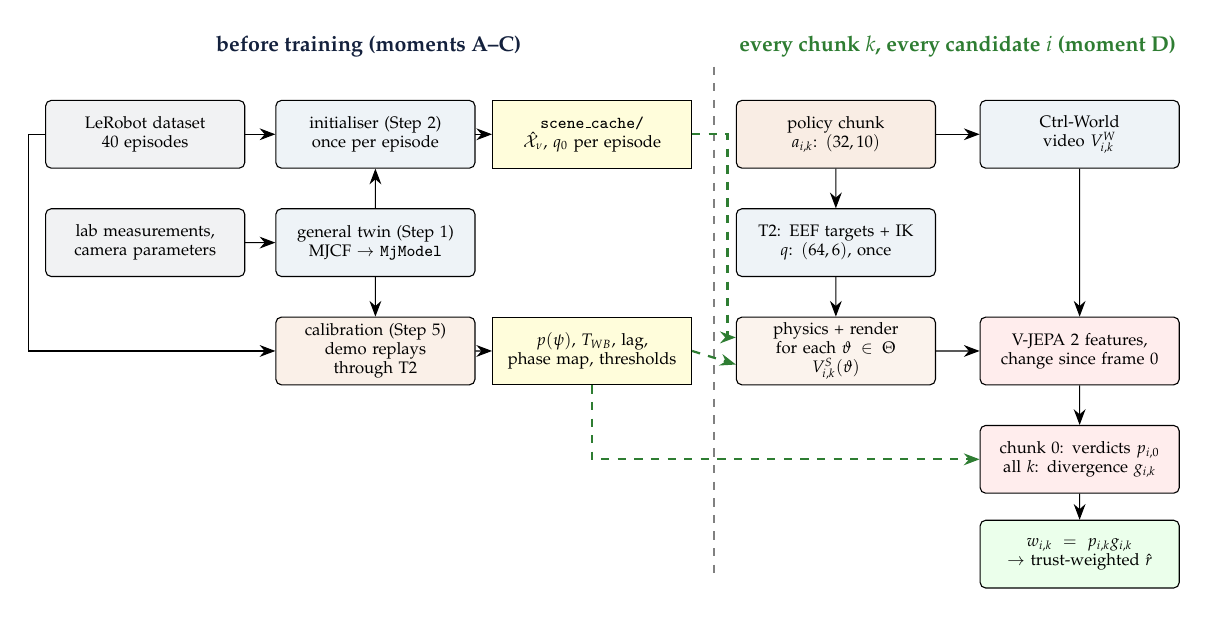
\begin{tikzpicture}[scale=0.86,transform shape,>={Stealth[length=2mm]},
  st/.style={draw,rounded corners=2pt,align=center,font=\scriptsize,minimum height=10mm,text width=28mm,inner sep=2pt},
  file/.style={draw,align=center,font=\scriptsize,fill=yellow!14,text width=28mm,inner sep=2pt,minimum height=10mm}]
% headers
\node[font=\small\bfseries,text=navy] at (3.3,1.3) {before training (moments A--C)};
\node[font=\small\bfseries,text=okgreen] at (12.0,1.3) {every chunk $k$, every candidate $i$ (moment D)};
\draw[gray,dashed] (8.4,1.0) -- (8.4,-6.6);
% offline
\node[st,fill=navy!6] (ds) at (0,0) {LeRobot dataset\\ 40 episodes};
\node[st,fill=blue!8] (ini) at (3.4,0) {initialiser (Step 2)\\ once per episode};
\node[file] (cache) at (6.6,0) {\texttt{scene\_cache/}\\ $\hat\X_\nu$, $q_0$ per episode};
\node[st,fill=navy!6] (lab) at (0,-1.6) {lab measurements,\\ camera parameters};
\node[st,fill=blue!8] (gen) at (3.4,-1.6) {general twin (Step 1)\\ MJCF $\to$ \texttt{MjModel}};
\node[st,fill=orange!10] (cal) at (3.4,-3.2) {calibration (Step 5)\\ demo replays through T2};
\node[file] (calf) at (6.6,-3.2) {$p(\psi)$, $T_{WB}$, lag,\\ phase map, thresholds};
\draw[->] (ds) -- (ini); \draw[->] (ini) -- (cache);
\draw[->] (lab) -- (gen); \draw[->] (gen) -- (ini); \draw[->] (gen) -- (cal);
\draw[->] (ds.west) -- ++(-0.25,0) |- (cal.west);
\draw[->] (cal) -- (calf);
% online
\node[st,fill=orange!12] (pol) at (10.2,0) {policy chunk\\ $a_{i,k}$: $(32,10)$};
\node[st,fill=blue!8] (cw) at (13.8,0) {Ctrl-World\\ video $\VW_{i,k}$};
\node[st,fill=blue!8] (t2) at (10.2,-1.6) {T2: EEF targets + IK\\ $q$: $(64,6)$, once};
\node[st,fill=orange!8] (sim) at (10.2,-3.2) {physics + render\\ for each $\vartheta\in\Theta$\\ $\VS_{i,k}(\vartheta)$};
\node[st,fill=red!7] (feat) at (13.8,-3.2) {V-JEPA 2 features,\\ change since frame 0};
\node[st,fill=red!7] (ver) at (13.8,-4.8) {chunk 0: verdicts $p_{i,0}$\\ all $k$: divergence $g_{i,k}$};
\node[st,fill=green!8] (w) at (13.8,-6.2) {$w_{i,k}=p_{i,k}g_{i,k}$\\ $\to$ trust-weighted $\hat r$};
\draw[->] (pol) -- (cw); \draw[->] (pol) -- (t2); \draw[->] (t2) -- (sim);
\draw[->] (cw) -- (feat); \draw[->] (sim) -- (feat); \draw[->] (feat) -- (ver); \draw[->] (ver) -- (w);
% artefacts into the loop
\draw[->,thick,dashed,okgreen] (cache.east) -- (8.6,0) |- ([yshift=2mm]sim.west);
\draw[->,thick,dashed,okgreen] (calf.east) -- ([yshift=-2mm]sim.west);
\draw[->,thick,dashed,okgreen] (calf.south) |- (ver.west);
\end{tikzpicture}
\caption{The whole flow. Left: what is built and saved before training. Right: what runs in every chunk. Dashed green arrows: saved artefacts read inside the loop (the cache and $p(\psi)$ set up the twins; the phase map and thresholds feed the verdicts).}
\label{fig:flow}
\end{figure}

\subsection{A walk through one episode}
Take a group whose start is training episode 3, and follow candidate $i$.
\begin{enumerate}
\item \textbf{Reset.} The env loads episode 3's first frame from the dataset (\code{CtrlWorldEnv.reset}). The twin plugin reads \code{scene\_cache\/episode\_003.json}: $q_0$ and, say, $M=4$ near-optimal laptop states. It builds $\Theta$ with $K=4$ samples of $\psi$ (16 elements), writes each $x_0$ and $q_0$ into its \code{MjData.qpos}, and sets the open-loop EEF state to the one the env uses.
\item \textbf{Chunk 0.} The policy outputs $a_{i,0}$, a $(32,10)$ array. Ctrl-World predicts $\VW_{i,0}$. In parallel the session converts $a_{i,0}$ once to 64 joint targets $(64,6)$ and runs the 16 twins: $64\times16$ physics steps each, recording the lid angle and contacts, and rendering the frames that the feature windows need. For probed candidates, the probe $\tilde a$ and the null action go through the same twins, and Ctrl-World is re-run from its saved state (\cref{sec:integration}).
\item \textbf{Compare.} V-JEPA 2 embeds the Ctrl-World clip and each twin clip; each is turned into change features (minus its own first-frame feature). Chunk 0 gives the per-action verdict and $p_{i,0}$; every chunk gives $S_{i,k}=\min_\vartheta d_{i,k}(\vartheta)$, the spread $\kappa_{i,k}$, and possibly the divergence chunk $k^\ast_i$.
\item \textbf{Chunks 1--4.} The twins continue from their \emph{own} states (never from Ctrl-World's frames), with the next actions. The EEF state carried forward is the same \code{next\_state} Ctrl-World uses.
\item \textbf{Weights.} $w_{i,k}=p_{i,k}\,g_{i,k}$ for $k=0..4$, attached to the rollout and used in the trust-weighted advantages.
\end{enumerate}

\subsection{How big is this?}\label{sec:size}
One rendered view at $192\times320$ RGB is $192\cdot320\cdot3\approx184$\,kB. One chunk of 64 frames, 3 views, is about 35\,MB per twin; for $|\Theta|=16$ twins about 570\,MB per candidate and chunk. That is why renders are \emph{streamed} into the feature encoder and never stored, and why the cheap reductions of the plan matter: render only the frames the V-JEPA windows use, fewer views or a lower resolution for the comparison, or $|\Theta|=8$. Physics itself is cheap (milliseconds per frame on CPU \chk); the render time per frame is measured in T0 and decides the in-loop budget.

%=====================================================================
\section{How it plugs into the training code}\label{sec:integration}
%=====================================================================
\subsection{The plugin mechanism}
The vendored runtime in \code{third\_party/} is not edited. The repo already has a pattern for adding behaviour at run time: \code{stage15\_plugin/}.
\begin{itemize}
\item \code{stage15\_plugin\/sitecustomize.py} is imported automatically by Python at start-up when its folder is on \code{PYTHONPATH}. It does nothing unless the environment variable \code{RLINF\_STAGE15\_MODE} is set; then it calls \code{install()} from \code{stage15\_hook.py}, which replaces selected functions of the runtime (\emph{monkeypatching}), and fails loudly if that does not work.
\item \code{stage15\_plugin\/launch\_ray\_node.sh} prepends the plugin folder to \code{PYTHONPATH} on each Ray node (line~89), so every worker process gets it.
\end{itemize}
The twin follows the same pattern \planned{} (roadmap WP 5.1): \code{twin\_plugin\/sitecustomize.py}, gated by \code{RLINF\_TWIN\_MODE} $\in\{$\code{off}, \code{log}, \code{weight}$\}$, and \code{RLINF\_TWIN\_ARM} selecting the training arm (T, T0, TG, S).

\begin{newc}{monkeypatching}
Replacing a function or method of an already imported module by another one at run time, e.g.\ \code{CtrlWorldEnv.chunk\_step = wrapped\_chunk\_step}. The wrapper usually calls the original and adds work before or after it. It keeps the thesis code separate from the vendored code, at the price of depending on the exact names of the patched functions.
\end{newc}

\subsection{Where each piece hooks in}
\begin{figure}[p]
\centering
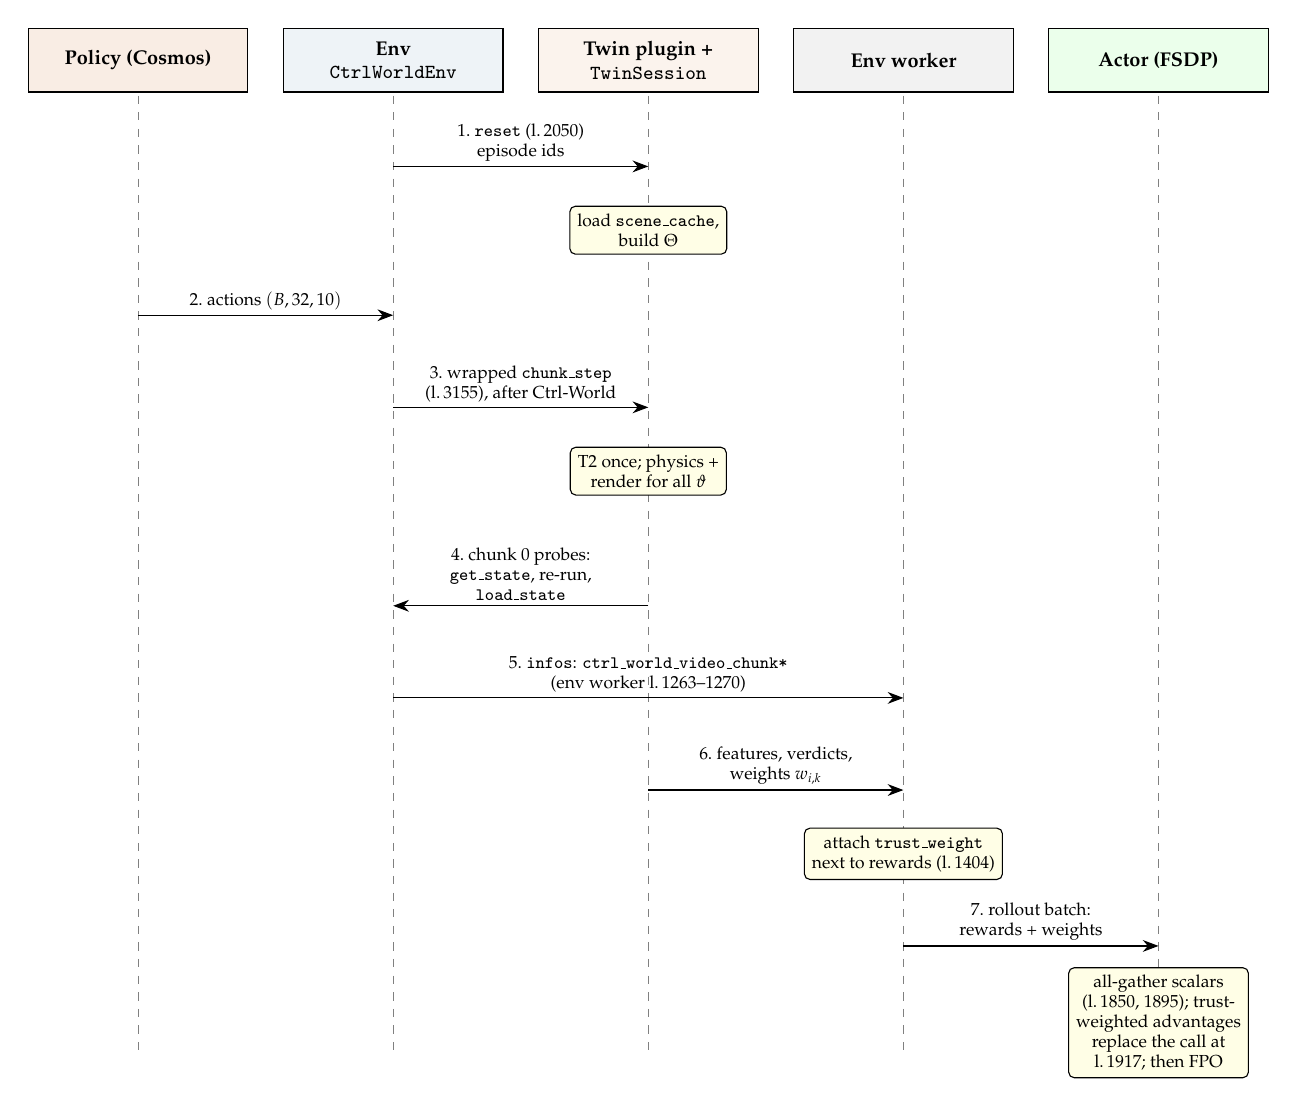
\begin{tikzpicture}[scale=0.9,transform shape,>={Stealth[length=2mm]},
  lane/.style={draw,fill=#1,minimum width=31mm,minimum height=9mm,font=\footnotesize\bfseries,align=center},
  msg/.style={font=\scriptsize,align=center,anchor=south,inner sep=2pt},
  note/.style={draw,rounded corners=2pt,fill=yellow!10,font=\scriptsize,align=center,inner sep=3pt}]
\node[lane=orange!12] (P) at (0,0) {Policy (Cosmos)};
\node[lane=blue!8] (E) at (3.6,0) {Env\\ \texttt{CtrlWorldEnv}};
\node[lane=orange!8] (T) at (7.2,0) {Twin plugin +\\ \texttt{TwinSession}};
\node[lane=gray!10] (W) at (10.8,0) {Env worker};
\node[lane=green!8] (A) at (14.4,0) {Actor (FSDP)};
\foreach \x in {0,3.6,7.2,10.8,14.4}{ \draw[gray,dashed] (\x,-0.5) -- (\x,-14.0); }
\draw[->] (3.6,-1.5) -- node[msg]{1.\ \texttt{reset} (l.\,2050)\\ episode ids} (7.2,-1.5);
\node[note] at (7.2,-2.4) {load \texttt{scene\_cache},\\ build $\Theta$};
\draw[->] (0,-3.6) -- node[msg]{2.\ actions $(B,32,10)$} (3.6,-3.6);
\draw[->] (3.6,-4.9) -- node[msg]{3.\ wrapped \texttt{chunk\_step}\\ (l.\,3155), after Ctrl-World} (7.2,-4.9);
\node[note] at (7.2,-5.8) {T2 once; physics +\\ render for all $\vartheta$};
\draw[->] (7.2,-7.7) -- node[msg]{4.\ chunk 0 probes:\\ \texttt{get\_state}, re-run,\\ \texttt{load\_state}} (3.6,-7.7);
\draw[->] (3.6,-9.0) -- node[msg]{5.\ \texttt{infos}: \texttt{ctrl\_world\_video\_chunk*}\\ (env worker l.\,1263--1270)} (10.8,-9.0);
\draw[->] (7.2,-10.3) -- node[msg]{6.\ features, verdicts,\\ weights $w_{i,k}$} (10.8,-10.3);
\node[note] at (10.8,-11.2) {attach \texttt{trust\_weight}\\ next to rewards (l.\,1404)};
\draw[->] (10.8,-12.5) -- node[msg]{7.\ rollout batch:\\ rewards + weights} (14.4,-12.5);
\node[note,anchor=north] at (14.4,-12.8) {all-gather scalars\\ (l.\,1850, 1895); trust-\\weighted advantages\\ replace the call at\\ l.\,1917; then FPO};
\end{tikzpicture}
\caption{Sequence of one chunk with the twin. Line numbers refer to commit \code{f4f669e}: env = \code{RT\/envs\/world\_model\/world\_model\_ctrl\_world\_env.py}; env worker = \code{RT\/workers\/env\/env\_worker.py}; actor = \code{RT\/workers\/actor\/fsdp\_actor\_worker.py}.}
\label{fig:seq}
\end{figure}

\begin{enumerate}
\item \textbf{Reset} (\code{CtrlWorldEnv.reset}, line~2050) knows which episode each environment starts from (\code{episode\_indices}). The plugin wraps it to reset the matching \code{TwinSession} from the cache.
\item \textbf{Every chunk} (\code{CtrlWorldEnv.chunk\_step}, line~3155) receives the policy's actions \code{[B, chunk, action\_dim]} and runs Ctrl-World through \code{\_infer\_next\_chunk\_frames} (line~2747). The wrapper calls the original, then steps the twins with the same actions. (The subclass \code{CosmosSelfFeedbackCtrlWorldEnv} calls \code{super().chunk\_step}, so wrapping the base method covers it \chk.)
\item \textbf{Probes at chunk 0} need Ctrl-World to predict again from the same state with another action and chosen seeds: \code{get\_state()} (line~3444) serialises the env, including the noise generator state; \code{load\_state()} (line~3508) restores it. Whether this restore is exact is assumption M4, tested first (roadmap WP 4.1).
\item \textbf{Ctrl-World's video} leaves the env in \code{infos} under \code{ctrl\_world\_video\_chunk}, \code{\_wrist}, \code{\_extra} (read in \code{env\_worker.py}, lines~1263--1270); this is where the comparison gets $\VW$.
\item \textbf{Weights} travel with the rewards. The actor gathers only \emph{scalar} per-step records across ranks (\code{\_compute\_cross\_rank\_grpo\_advantages}, line~1716; \code{all\_gather} at lines~1850 and~1895--1896), because a group of 16 is spread over 4 ranks. The weight becomes one more scalar column of that gather, and the trust-weighted function (roadmap WP 1.2) replaces the call to \code{validate\_and\_compute\_group\_suffix\_advantages} (\code{RT\/algorithms\/cross\_rank\_grpo.py}, line~801; called at line~1917).
\end{enumerate}

\textbf{First mode: log only.} In \code{log} mode the plugin computes everything and logs verdicts, scores, spreads and weights, but forces $w\equiv1$. Its acceptance test is that advantages are bit-identical to the baseline. This is also arm A of the proposal (E1, E2): the audit runs on the original method.

\subsection{Where things run}
\begin{center}\small
\begin{tabularx}{\linewidth}{@{}>{\raggedright\arraybackslash}p{4.2cm}>{\raggedright\arraybackslash}p{3.6cm}>{\raggedright\arraybackslash}X@{}}
\toprule
\textbf{Part} & \textbf{Hardware} & \textbf{Note}\\
\midrule
Ctrl-World, Cosmos, V-JEPA 2 & GPU & unchanged, plus probe re-runs at chunk 0 (+25--50\% Ctrl-World calls)\\
T2 (EEF targets, IK) & CPU & once per candidate and chunk, shared by all $\vartheta$\\
MuJoCo physics, rendering & CPU (EGL on GPU nodes \chk) & $|\Theta|$ rollouts per candidate, in parallel\\
Initialiser, calibration & any GPU machine, offline & before training; results cached\\
\bottomrule
\end{tabularx}
\end{center}

%=====================================================================
\section{Status and what comes next}\label{sec:status}
%=====================================================================
\begin{center}\small
\begin{tabularx}{\linewidth}{@{}>{\raggedright\arraybackslash}p{4.0cm}>{\raggedright\arraybackslash}p{2.9cm}>{\raggedright\arraybackslash}X@{}}
\toprule
\textbf{Component} & \textbf{Status} & \textbf{Next step (roadmap WP)}\\
\midrule
Conventions, transforms & \done & --\\
Robot FK and MJCF (T1) & \done & fix the Linux/Windows 1-ulp asset test (WP 1.1)\\
Actions $\to$ EEF $\to$ joints (T2) & \done{} synthetic & demo check when the dataset arrives (Phase 6)\\
Headless render (T0) & not started & WP 1.1\\
Laptop scene, physics (T3) & \skel & WP 2.3, with placeholder geometry\\
Cameras, masks (T4) & \skel & WP 3.1; real values from the lab or WP 3.3\\
Initialiser (T5) & \skel & WP 3.2 on synthetic renders, then real frames\\
Calibration (Step 5) & \planned & WP 1.5 (rules), WP 3.4 (identifiability), then demos\\
Session with $\Theta$ (T7) & \skel{} (kinematics only) & after T3 and T4\\
Plugin, logging & \planned & WP 5.1, 5.2\\
\bottomrule
\end{tabularx}
\end{center}
\code{progress.md} (17 Nov) reports 18 T1 tests and 35 T2 tests passing; on Linux, two T1 asset tests fail because of a known 1-ulp difference between the Windows and Linux maths libraries (fix in WP 1.1).

\appendix
%=====================================================================
\section{Shapes cheat sheet}
%=====================================================================
\begin{center}\small
\begin{tabularx}{\linewidth}{@{}>{\raggedright\arraybackslash}p{4.3cm}>{\raggedright\arraybackslash}p{5.0cm}>{\raggedright\arraybackslash}X@{}}
\toprule
\textbf{Object} & \textbf{Shape / type} & \textbf{Code}\\
\midrule
Policy action chunk & $(32,10)$ float, 15\,Hz & input of \code{ActionsToJoints.step\_chunk}\\
EEF state & 7 numbers: $[x,y,z,r_x,r_y,r_z,g]$ in $W$ & \code{EEFTargets.next\_state}\\
EEF targets for Ctrl-World/twin & $(64,7)$, 30\,Hz & \code{EEFTargets.ctrl\_states}\\
Joint targets & $(64,6)$ rad & \code{JointChunk.q}\\
Pose & $(4,4)$ float64 & \code{fk}, \code{make\_T}\\
Scene state $x$ & $(p_x,p_y,\text{yaw},\vartheta)$ + $q$ & \code{SceneState}\\
Per-chunk physics record & lid angle and contact flags, 64 values each & \code{ChunkRollout}\\
One render & $(192,320,3)$ \code{uint8} per camera & \code{TwinRenderer.render}\\
Uncertainty set & $|\Theta|=K\cdot M\approx16$ (model, data) pairs & \code{TwinSession} (planned)\\
Per-episode fit & JSON & \code{scene\_cache\/episode\_XXX.json}\\
Trust weight & one float per candidate and chunk & plugin $\to$ actor gather\\
\bottomrule
\end{tabularx}
\end{center}

\section{Glossary}
\begin{center}\small
\begin{tabularx}{\linewidth}{@{}>{\raggedright\arraybackslash}p{3.6cm}X@{}}
\toprule
\textbf{Term} & \textbf{Meaning here}\\
\midrule
general twin $\mathcal T$ & robot, table, laptop model, cameras and $p(\psi)$: everything common to all start scenes of a task\\
MJCF / \code{MjModel} / \code{MjData} & scene description (XML) / compiled constants / one simulation's state\\
$\psi$, $p(\psi)$ & uncertain physics parameters and their belief (samples); stored in models\\
$x_0$, $\hat\X_\nu$ & laptop start state and the set of near-optimal fits; stored in \code{qpos}\\
$\vartheta=(\psi,x_0)$, $\Theta$ & one plausible twin; all of them\\
$T_{WB}$ & base of the robot in the frame of recorded poses; estimated from demos\\
TCP & tool centre point, 0.18\,m beyond the flange\\
IK, Jacobian, DLS & inverse kinematics; linearisation of FK; damped least squares\\
render-and-compare & fit by rendering guesses and scoring overlap with observed masks\\
position actuator & MuJoCo motor that pulls a joint towards a target angle with a spring--damper\\
monkeypatching & replacing a function of an imported module at run time\\
\bottomrule
\end{tabularx}
\end{center}

\end{document}
